\chapter{Design ESB in Openshift}
\label{cha:esboc}
In this chapter, the ESB integration as discussed in Section \vref{sec:esb-integration-example}, will be designed as microservices, which can run on a Openshift Cluster. A Openshift Project will act as the ESB, which will provide the orchestration, mediation, configurations and secrets for the integration services. The concrete functionality of the services is considered not to be important. The goal is to redesign the Service Components of Figure \vref{fig:esb-design-sca} as microservices, and to design the Openshift Project, which will host the integration services.
\\ \\
As discussed in Chapter \vref{cha:esb}, an ESB is a distributed computing architecture, where distributed services act as a consumer or producer. These integration services provide a business value for an enterprise in form of an integration of an internal or external service. There are multiple providers of ESB middleware like JBoss Fuse, which provide tooling for implementing Service Components running on an ESB. The prototype will illustrate that SOA Service Components can be implemented as microservices, where features provided by the ESB middleware such as mediation and bindings will have to be replaced by other implementations.

\section{Microservice Architecture}
Figure \vref{fig:esboc-design-services} illustrates the microservice architecture of the integration prototype, based on the architecture of Figure \vref{fig:esb-design-sca}. Conceptually, the transformation of a Service Component to a microservice is easy, because a Service Component and a microservice act very similar. Compared to a Service Component of a ESB middleware, a microservice is completely separated from the other services, brings in its own dependencies and runs in its own runtime environment. From the implementation point of view, the microservice needs to provide an runtime environment, which formerly was provided by the ESB middleware. Therefore, that the microservices are completely separated, the access of other services is not mediated as usual anymore, because the communication is now performed via standard protocols like HTTP(S). In a monolithic ESB application running on EAP, every Service Component accessed via a Reference uses the actual service instance within the same runtime environment. With microservices, running in their own runtime environment, it is not possible to access the service instance directly anymore. Only communication via standard protocols such as HTTP(S) is supported.

\begin{figure}[htbp]
	\centering
	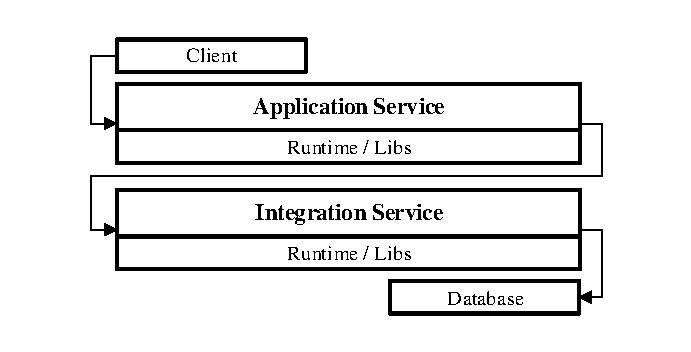
\includegraphics[scale=1]{images/esboc-design-microservice.pdf}
	\caption{Microservice Architecture}
	\label{fig:esboc-design-services}
\end{figure}

\section{Microservice Aspects}
\label{sec:esboc-aspects}
In this section the necessary aspects of microservices are discussed, which will ensure that the integration services are properly implemented and can effortlessly be managed. Especially the monitoring of the integration services becomes very important when moving from a conventional monolithic ESB application, like an application running on JBoss Fuse, to microservice based integration services. Integration services running as microservices on Openshift, are running in their own runtime environment and therefore cannot share any runtime resources, which are available in a monolithic application. 
\\ \\
Figure \vref{fig:esboc-aspects} illustrates the hierarchy of the microservice aspects, which are discussed in the following sections. The in the following discussed microservice aspects shall ensure that the microservices are 
\begin{itemize}
	\item secure,
	\item configurable for multiple environments,
	\item observable by developers and operators,
	\item resilient to failures
	\item and measurable.
\end{itemize}

\begin{figure}[htbp]
	\centering
	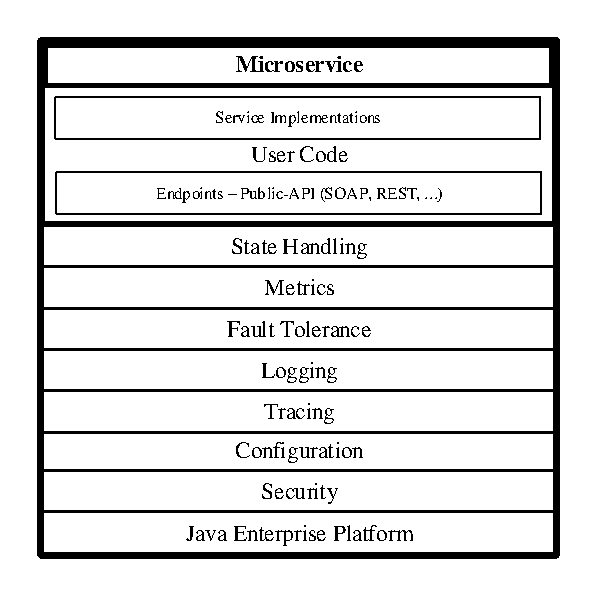
\includegraphics[scale=1]{images/esboc-requirement-services.pdf}
	\caption{Service Requirements}
	\label{fig:esboc-aspects}
\end{figure} 

\subsection{Security}
\label{sec:esboc-aspects-security}
Distributed microservices need to be secured properly from unauthorized access, therefore the microservices will be secured with OAuth. OAuth is a token based authentication scheme, which has become popular over past few years. There are several open source implementations for interacting with a authentication service via the OAuth scheme. The Integration Service must authenticate its client the Application Service against an central authentication service, whereby the Application Service will retrieve the access tokens from the central authentication service \cite{OAuth2018}.

\subsection{Configuration}
\label{sec:esboc-aspects-config}
The MicroProfile specifications provide the MicroProfile-Config specification, which provides an API to inject configuration parameters into objects. The injected configuration parameters are loaded from so called configuration sources. A configuration source can either be Java System-Properties, Environment Variables, Properties Files, YAML Files or custom implementations for instance to retrieve configurations from a database. The microservices must be implemented in a way to be configurable for different stages such as DEV (development), TEST (testing) and PROD (productive environment), whereby  the services are only allowed to use configuration parameters via injection  \cite{EclipseMicroprofileConfig2018}.

\subsection{Tracing}
\label{sec:esboc-aspects-tracing}
The MicroProfile specifications provides the OpenTracing specification, which provides an API for tracing an application on a method level or across service boundaries. Distributed Tracing allows to comprehend service or method call chains of distributed services. There is open source tooling available to analyze the collected tracing data provided by the distributed services. The services must collect reasonable tracing information and send this data to a central tracing service \cite{CNCFOpentracing2018}.

\subsection{Logging}
\label{sec:esboc-aspects-logging}
Distributed Logging allows to comprehend logs across service boundaries within a service call chain, where the logs of all involved services have to be marked with the same transaction id. There is open source tooling available to analyze the collected logs. The services must provide all of their logging to a central service, whereby the logs are marked with a transaction id, which is provided by the OpenTracing API. Optionally, the services are allowed to add additional markers, which can help developers and operators to analyze problems or to group service logs.

\subsection{Metrics}
\label{sec:esboc-aspects-metrics}
The MicroProfile specifications provide the specification MicroProfile-Metrics, which provides an API to define and manage metrics. Metrics allow to comprehend the state of a microservice such as resource consumption, REST-API calls or Failure counts. Metrics along with distributed tracing and distributed logging, provide the necessary data, operators need to analyze failures in services, which occurred in service call chains. The services must provide and publish metrics, which can be made available to a central metric service.

\subsection{Fault Tolerance}
\label{sec:esboc-requirements-service-fault}
The MicroProfile specifications provide the specification MicroProfile-Fault-Tolerance, which provides an API to define fault tolerance behavior such as retries, timeouts and error fall-backs. The fault tolerance of a service means, that if a depending service is not accessible at the time, a service must not fail immediately after the first try, but the service should retry to call the depending service for several times, and fail when all retries have failed. Such a behavior ensures that short timed communication errors, redeployments or overloads do not immediately cause a service to fail. The services must provide proper fault tolerance configuration and fall-back behavior to be able to recover from such errors in a proper manner. \cite{EclipseMicroprofileFault2018}.   

\subsection{API Management}
\label{sec:esboc-requirements-service-api}
The API management of a public API such as REST-API and REST-Models ensure that the clients, using a public API, are not broken by changes made on that API. There are several opinions on how API management can be done. A public API has to be stable per design, and needs to evolve and provide backward compatibility in a way, so that clients have enough time to catch up with the changes. Swagger has become very popular for documenting REST-API, where the documentation can be used to generate clients, provide documentation for developers and to test the public API. The services must be capable of migrating their public API in a way that the clients are not broken by made changes and need to publish the Swagger definitions of their public REST-API. \cite{SmartBearSwagger2018, RestVersion2018}.

\section{Openshift Architecture}
\label{sec:esboc-design-oc}
Figure \vref{fig:esboc-design-openshift-project} illustrates the design of the Openshift Project, which will host the integration services. As discussed in Section \vref{sec:paas-openshift}, Openshift isolates the namespaces, by bringing in the concept of an Openshift Project. Services hosted in an Openshift Project which are not exposed via an Openshift Route, are implicitly protected from external access from the Internet or services hosted in other Openshift Projects. The Openshift Project will contain the Application Service, the Database Service and the Integration Service. The Application Service has access to the Internet and will be accessed by the Client from the Internet via its public address. The Integration Service and the Database Service are not exposed to the Internet and can only be accessed within the Openshift Project by their service names.

\begin{figure}[htbp]
	\centering
	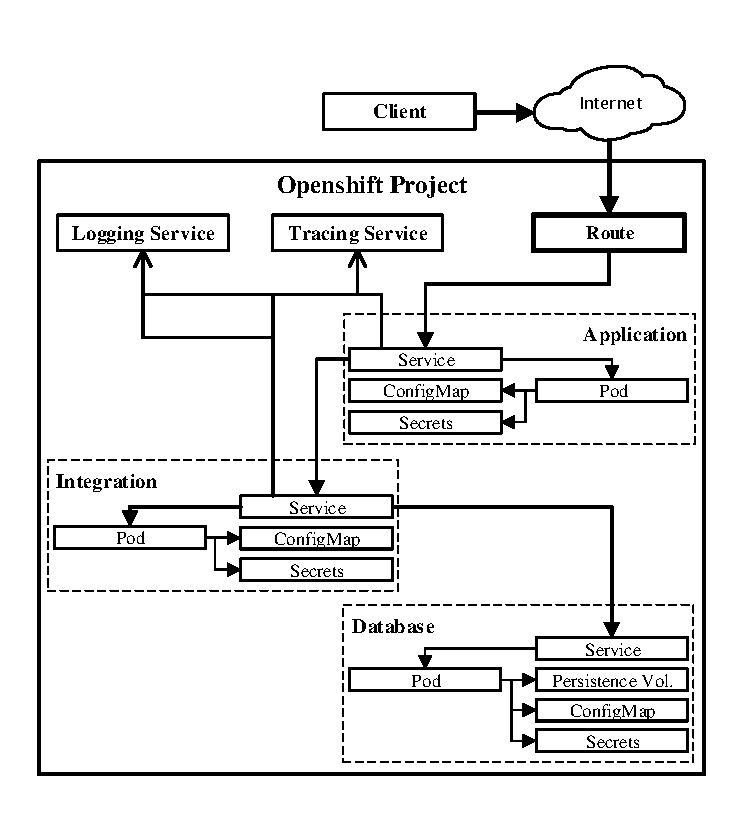
\includegraphics[scale=1]{images/esboc-design-openshift.pdf}
	\caption{Openshift Project architecture}
	\label{fig:esboc-design-openshift-project}
\end{figure} 

The orchestration and mediation of the services are managed by Openshift, whereby the services communicate with each other via their service names, which ensures that the communication stays within the Openshift Project. If multiple service instances are present, then Openshift handles the request assignment via Round Robin. Openshift will provide the configurations and secrets referenced by the integration service templates to the services as configured.

\section{Openshift Requirements}
\label{sec:esboc-requirements-oc}
The implementation of the Openshift resources such as templates and scripts must be implemented under consideration of the principles of IaC, which has been discussed in Section \vref{sec:iac-principles}. Keeping to the principles of IaC will ensure, that the Openshift Project can effortlessly be managed.   
\\ \\
The Openshift Project will host the integration services and manage their configuration and secrets via Openshift ConfigMaps and Openshift Secrets, which have been discussed in Section \vref{sec:caas-kubernetes-objects}. The configurations and secrets are managed outside the microservice code bases and are provided by the hosting Openshift Project for a specific stage the Openshift Project represents. The configurations and secrets are supposed to be managed by operators and are only made available to the services during runtime and cannot be accessed by developers.
\\ \\
The integration services shall manage their integration into Openshift, by providing the necessary templates, whereby configurations and secrets are referenced by their predefined names and keys. The integration service must expose all necessary configuration parameters, which allow to configure the integration service for a specific stage a Openshift Project represents.
\\ \\
For demonstration purpose the Openshift Project hosting the integration services, shall host a tracing service and a logging service as well. This is due to the fact, that in shared environments only HTTP(S) protocol is allowed, but tracing and logging data is usually send via UDP protocol. 
\\ \\
The next Chapter \vref{cha:esbi} will discuss the implementation of the in this chapter designed prototype. 
